

\chapter{考察}
\label{seq:considaration}
この章では,本研究で完成させることができなかった反射,屈折の法則の視覚化プログラムについて,現状の実装を記した上で,処理の問題点を考察する.

\section{反射の法則の視覚化}
\label{seq:reflection}
図\ref{fig:reflectionsetumei}は反射面に一定の間隔で配置された波源から生成される円形波の変位情報から反射角を描写するプログラムである.
\begin{figure}[H]
 \begin{center}
  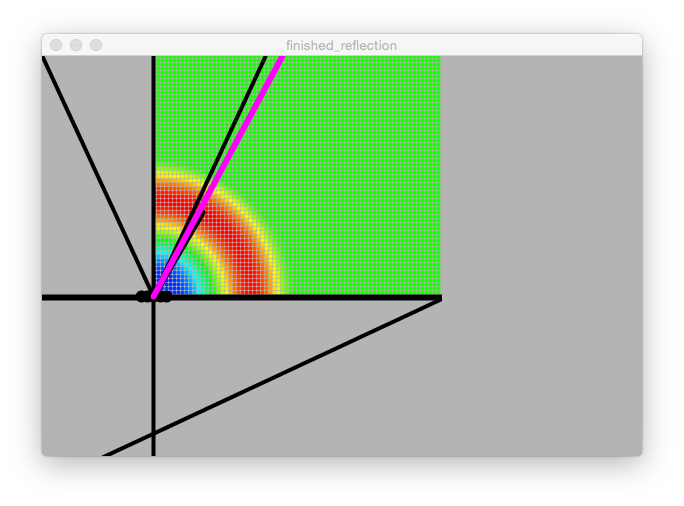
\includegraphics[width=110mm]{../result/reflectionsetumei.png}
 \end{center}
 \caption{プログラムの動作の様子.}
 \label{fig:reflectionsetumei}
\end{figure}

プログラムを起動すると図\ref{fig:reflectionincident}のように入射波となる平行波が画面左上から右下にかけて進んでくる.波源は入射波の速度に応じた間隔で5つ生成される.

入射角が20度の入射波によって各波源が生成され,それらから生じた波を描写したものが図\ref{fig:reflection20}である.図\ref{fig:reflection20}の画面右上の波の描写領域に注目すると3本の線がある.

画面の上端に届いていない黒線は,3個目の波源(入射角と反射角の境界線)から現在の最大変位を結んだものである.各フレームごとに最大変位が変わるため,この線もそれに応じて更新される.

赤線は各フレームごとの最大変位をとる座標の傾きを平均化して描写したものである.\ref{seq:pxcelproblem}節で詳しく取り扱うが,プログラムの仕様上,理論上の最大変位を取得することは出来ないので値を平均化することで精度を高める目的がある.

もう一つの黒線は,反射の法則を満たす角度で3個目の波源から引いた線である.この線と赤線のずれを無くすことを目標としていた.
\begin{figure}[H]
\begin{minipage}{0.5\hsize}
\begin{center}
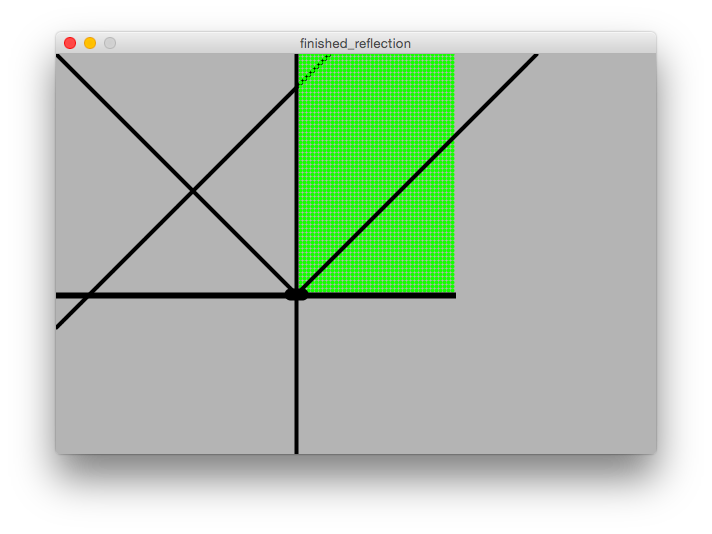
\includegraphics[width=\linewidth]
  {../result/reflectionincident.png}
\caption{入射波が進行する様子}
\label{fig:reflectionincident}
\end{center}
\end{minipage}%
\begin{minipage}{0.5\hsize}
\begin{center}
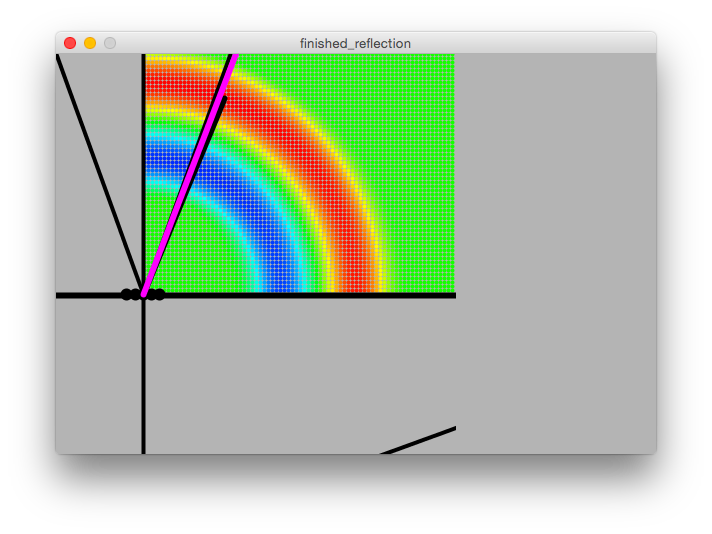
\includegraphics[width=\linewidth]
  {../result/reflectionangle20.png}
\caption{入射角を$20^{\circ}$に設定した波が進行する様子.}
\label{fig:reflection20}
\end{center}
\end{minipage}
\end{figure}

入射波を$20^{\circ}$に設定した結果が図\ref{fig:reflection20finish}, $40^{\circ}$に設定した結果が図\ref{fig:reflection40finish}である.
\begin{figure}[H]
\begin{minipage}{0.5\hsize}
\begin{center}
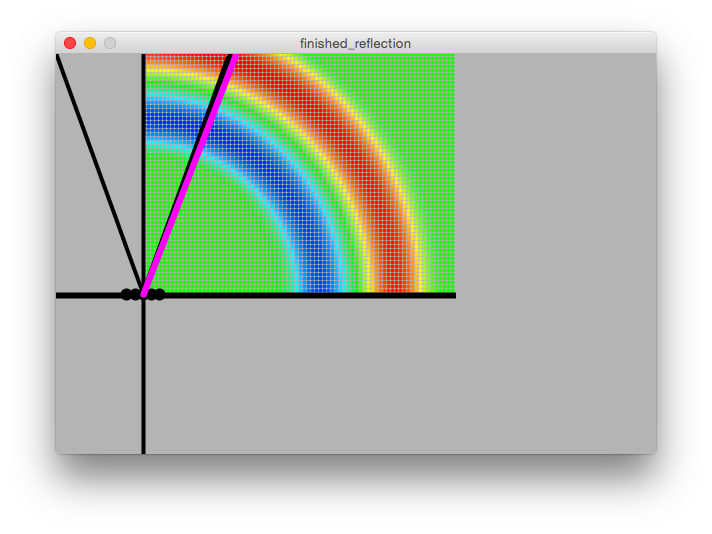
\includegraphics[width=\linewidth]
  {../result/finishreflectionangle20.png}
\caption{入射角が$20^{\circ}$の時の反射角の結果.}
\label{fig:reflection20finish}
\end{center}
\end{minipage}%
\begin{minipage}{0.5\linewidth}
\begin{center}
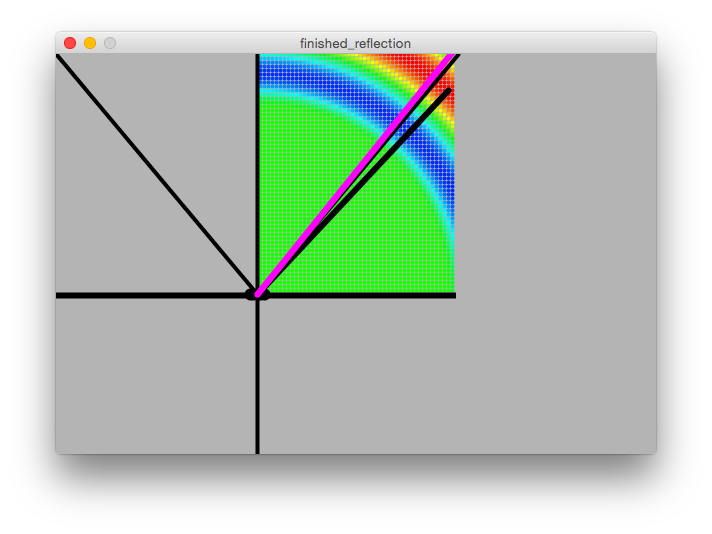
\includegraphics[width=\linewidth]
  {../result/finishreflectionangle40.png}
\caption{入射角が$40^{\circ}$の時の反射角の結果.}
\label{fig:reflection40finish}
\end{center}
\end{minipage}
\end{figure}

図\ref{fig:reflection20finish},図\ref{fig:reflection40finish}を見ると僅かながらずれが生じており,本研究ではこのずれを修正することが出来なかった.
\section{屈折の法則の視覚化}
図\ref{fig:refraction}は屈折率が1.5の媒質に,入射角$30^{\circ}$の入射波が進行した際の屈折角の角度を示すプログラムである.
\begin{figure}[H]
 \begin{center}
  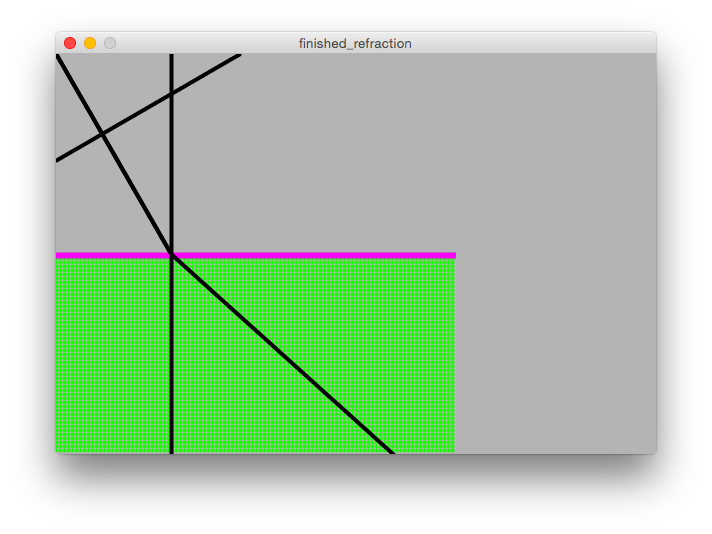
\includegraphics[width=130mm]{../result/refractionangle3015.png}
 \end{center}
 \caption{入射角に対する反射角の角度.}
 \label{fig:refraction}
\end{figure}

この後,媒質に応じた速度の素元波を発生させ,\ref{seq:reflection}節で用いた方法と同じ要領で屈折角を描写しようと考えていたが,反射角の描写が理論通りにできていないので,処理の実装に取り掛かることができなかった.


\section{最大変位の点へ線を引く理由}
\label{sec:hansyaarugorizumu}
\ref{seq:reflection}節で示したように,本研究では,波の最大変位を辿れば反射角,屈折角の角度となると考えてプログラムを構築した. この考えに至った理由を以下に示す.

当初,波の反射波,屈折波をリアルタイムで描写する方法が思いつかなかったため,入射波の角度に対して素元波がどのように広がっていくのかを描写するプログラムを作成し,糸口を探った. 入射角を$40^{\circ}$に設定したものが図\ref{fig:angle40},$50^{\circ}$に設定したものが図\ref{fig:angle50}である.

\begin{figure}[H]
\begin{minipage}{0.5\hsize}
\begin{center}
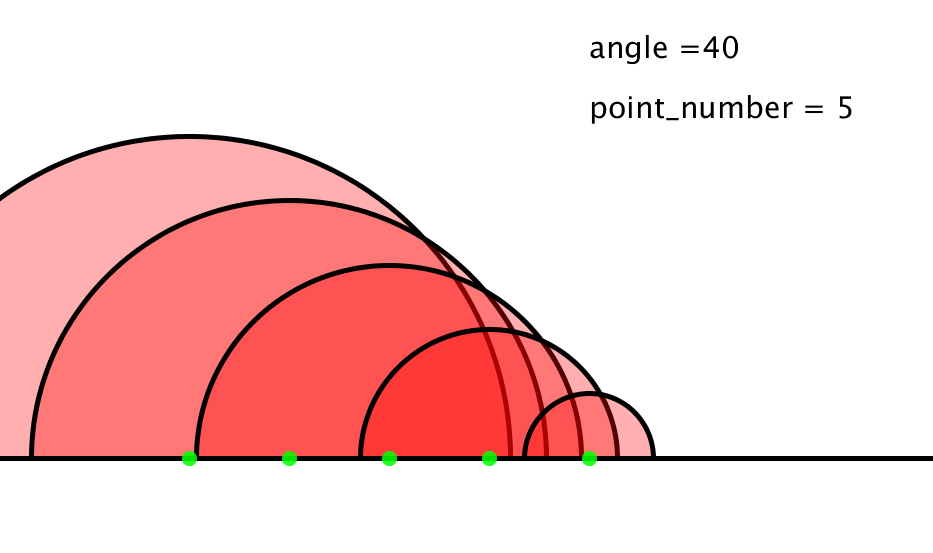
\includegraphics[width=70mm]
  {../considaration/angle40.png}
\caption{入射波 = $40^{\circ}$}
\label{fig:angle40}
\end{center}
\end{minipage}%
\begin{minipage}{0.5\hsize}
\begin{center}
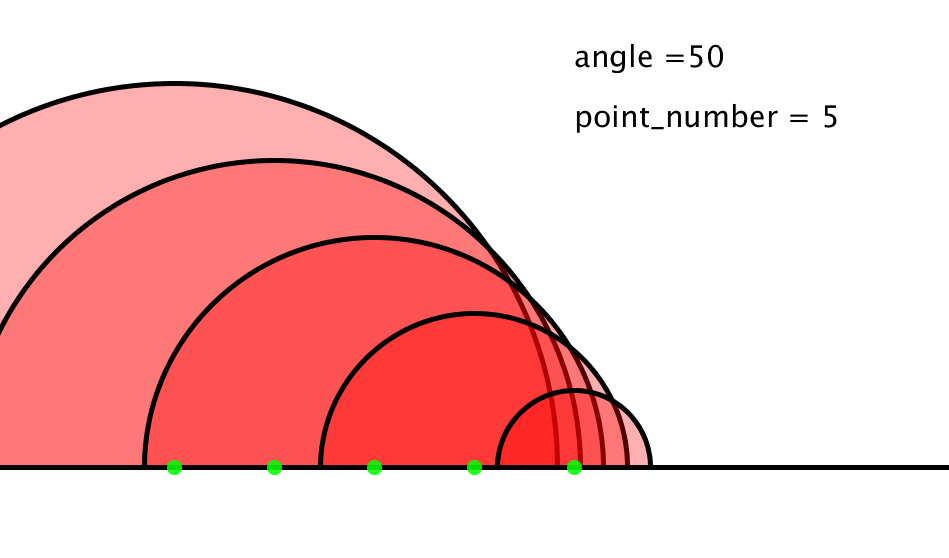
\includegraphics[width=70mm]
  {../considaration/angle50.png}
\caption{入射角 = $50^{\circ}$}
\label{fig:angle50}
\end{center}
\end{minipage}
\end{figure}
また図\ref{fig:angle50}の状態から一定時間経過した素元波を描写した図\ref{fig:angle50time}
を作成した.
\begin{figure}[H]
 \begin{center}
  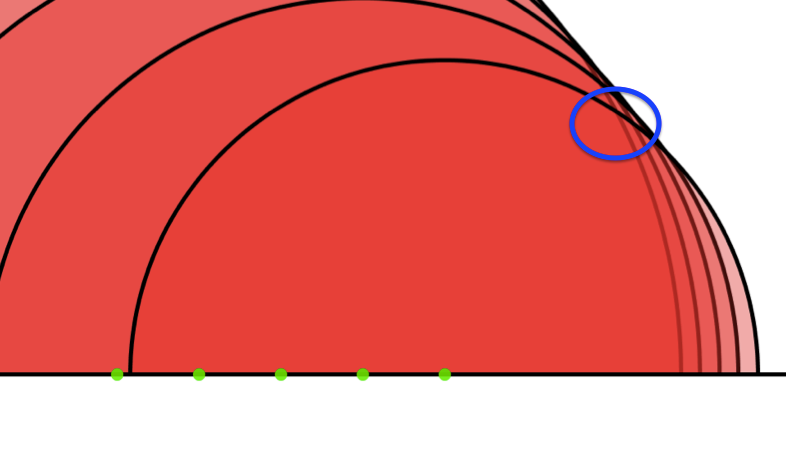
\includegraphics[width=130mm]{../considaration/angle50time.png}
 \end{center}
 \caption{図\ref{fig:angle50}から一定時間が経過した時の素元波.}
 \label{fig:angle50time}
\end{figure}
図\ref{fig:angle50time}の最大位相は青枠周辺だと考え,青枠と中心の波源を結ぶと,理想的な角度に近くなった.
よって毎フレームごとに擬似ピクセルの中から最も変位の値が大きいものを選び出し,そこに対して線を引くことで反射角,屈折角を表現すれば良いと考えた.
\section{アルゴリズムの問題点}
\ref{seq:reflection}節で示したように理論上の反射角と\ref{sec:hansyaarugorizumu}のアルゴリズムによって描写した反射角には若干のずれが生じる. そこでこの問題が生じる原因として2つの仮説を立てた.
\subsection{擬似ピクセルの問題}
\label{seq:pxcelproblem}
プログラムの実装上,擬似ピクセルの最小値は1であり,かつ整数値に限る. しかし本来の物理現象を考えると,波の最大変位の座標は整数であるとは限らない.図\ref{fig:pixcelproblem}の点Aが理論上の最大変位点とすると,点Aに線を引くことはできず,青点で示す各擬似ピクセルの左上の座標のいずれかにしか引くことができない. このずれが毎フレームごとに蓄積された結果,適切な結果が得られなかったと考えられる.
\begin{figure}[htbp]
 \begin{center}
  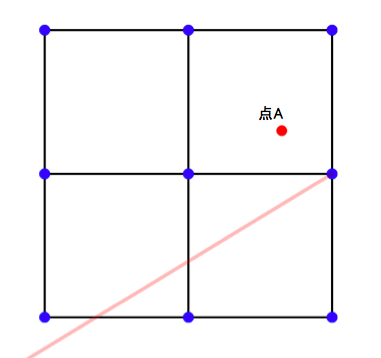
\includegraphics[width=70mm]{../considaration/pixcelproblem.png}
 \end{center}
 \caption{理論上の最大変位とプログラム上の最大変位の誤差.}
 \label{fig:pixcelproblem}
\end{figure}

\subsection{波源の個数の問題}
本研究で作成したプログラムは波源の数を5個に設定しているが,実際の物理現象を考えると波源は無限に存在する.
波源が無限に存在する故に波が反射や屈折を起こす際,素元波の共通接線と垂直に交わる線が新しい波面となる理論が成り立つが,プログラムでは波源の数は有限なのでこれが完璧には成り立たない.これが値のずれを生んでいるのではないかと考えられる.









